%\documentclass[portrait,final,a0paper,fontscale=0.292]{baposter}
\documentclass[portrait,a0paper,fontscale=0.31]{baposter}

\usepackage{calc}
\usepackage{graphicx}
\usepackage{amsmath}
\usepackage{amssymb}
\usepackage{relsize}
\usepackage{multirow}
\usepackage{rotating}
\usepackage{bm}
\usepackage{url}

% Redmar
\usepackage{enumitem}       %set indent for enumerate/itemize
\setitemize{leftmargin=0.3cm,itemsep=1.3em,parsep=0pt}%,topsep=0pt}
\usepackage[none]{hyphenat} %disables all hyphenation
%https://tex.stackexchange.com/questions/79591/superscripts-in-bibliography-with-bibtex
\usepackage[super]{natbib} 
\usepackage[font=small,labelfont=bf]{caption}
\DeclareCaptionFont{tiny}{\tiny}
%\usepackage{svg}
\usepackage{verbatim}

\usepackage{graphicx}
\usepackage{multicol}

%\usepackage{times}
%\usepackage{helvet}
%\usepackage{bookman}
\usepackage{palatino}

% Disable due to conflict with usepackage caption
%\newcommand{\captionfont}{\footnotesize}

\graphicspath{{images/}{../images/}}
\usetikzlibrary{calc}

%% Some names etc
\newcommand{\option}[1]{\texttt{#1}}
\newcommand{\exonviz}{\textbf{ExonViz} }
\newcommand{\senterica}{\textit{Salmonella enterica} serovar Heidelberg }
\newcommand{\heidelberg}{\textit{S.} Heidelberg }
\newcommand{\fcite}[2]{#1$^#2$}
\newcommand{\mdr}{multidrug-resistant }
\newcommand{\Mdr}{Multidrug-resistant }
\newcommand{\reference}{reference strain SL476 }
\newcommand{\amr}[2]{\textbf{#1} #2,}
\newcommand{\famr}[2]{\textbf{#1} #2.}
\newcommand{\cmy}{\textit{bla}{\tiny CMY-2}}
\newcommand{\padd}{\vspace*{0.2cm}}
\newcommand{\ppadd}{\vspace*{0.29cm}}

%%%%%%%%%%%%%%%%%%%%%%%%%%%%%%%%%%%%%%%%%%%%%%%%%%%%%%%%%%%%%%%%%%%%%%%%%%%%%%
%%% Begin of Document
%%%%%%%%%%%%%%%%%%%%%%%%%%%%%%%%%%%%%%%%%%%%%%%%%%%%%%%%%%%%%%%%%%%%%%%%%%%%%%

\begin{document}

%%%%%%%%%%%%%%%%%%%%%%%%%%%%%%%%%%%%%%%%%%%%%%%%%%%%%%%%%%%%%%%%%%%%%%%%%%%%%%
%%% Here starts the poster
%%%---------------------------------------------------------------------------
%%% Format it to your taste with the options
%%%%%%%%%%%%%%%%%%%%%%%%%%%%%%%%%%%%%%%%%%%%%%%%%%%%%%%%%%%%%%%%%%%%%%%%%%%%%%
% Define some colors

%\definecolor{lightblue}{cmyk}{0.83,0.24,0,0.12}
\definecolor{lightblue}{rgb}{0.145,0.6666,1}
\definecolor{darkblue}{rgb}{.082352,.2588235,.450980}
\definecolor{dcrtblue}{rgb}{0.29804,0.44706,0.71765} % #4C72B7
\definecolor{dcrtgreen}{rgb}{0.56078, 0.61176, 0.35294} % #8F9C5A
\definecolor{dcrtyellow}{rgb}{0.83137, 0.68235, 0.16863} % #D4AE2B
\definecolor{dcrtorange}{rgb}{0.8549,0.45882,0.32549} % #DA7553

%\hyphenation{resolution occlusions}
%%
\begin{poster}%
  % Poster Options
  {
  % Show grid to help with alignment
  grid=false,
  % Column spacing
  colspacing=2em,
  % Color style
  bgColorOne=white,
  bgColorTwo=white,
  %borderColor=lightblue,
  borderColor=white,
  headerColorOne=dcrtgreen,
  headerColorTwo=dcrtgreen,
  headerFontColor=white,
  boxColorOne=white,
  boxColorTwo=dcrtblue,
  % Format of textbox
  textborder=faded,
  % Format of text header
  eyecatcher=true,
  headerborder=closed,
  headerheight=0.1\textheight,
%  textfont=\sc, An example of changing the text font
  headershape=rounded,
  headershade=shadelr,
  headerborder=open,
  headerfont=\Large\sf\bf, %Sans Serif
  headerheight=0.13\textheight,
  textfont={\setlength{\parindent}{1.5em}},
  boxshade=plain,
%  background=shade-tb,
  background=plain,
  linewidth=2pt,
  }
  % Eye Catcher
  %{\includegraphics[height=5em]{images/nvwa.png}} 
  {}
  % Title
  {
    {
      ExonViz: An application to visualize transcripts and variants
    }
    %\vspace{0.3em}
  }
  % Authors
  {
    %\vspace{0.15em}
    {
      \fcite{Redmar R. van den Berg}{{1,2}}, \fcite{Marlen C. Lauffer}{{1,2}}, \fcite{Jeroen F.J. Laros}{{2}}
      \\{\smaller $^1$ \textit{Dutch Center for RNA Therapeutics}}
      \\{\smaller $^2$ \textit{Department of Human Genetics, Leiden University Medical Center, Leiden, The Netherlands}}
    }
    %\vspace{0.15em}
  }
  %{Netherlands Food and Consumer Product Safety Authority}
  % University logo
  %{\includegraphics[height=10.5em]{images/rijksoverheid3.png}} 
  %{\includegraphics[height=9.5em]{images/rijksoverheid3.png}} 
  % {\parbox[top][12em][t]{5em}{
\includegraphics[height=9.5em]{images/rijksoverheid4.png}}} 

%%%%%%%%%%%%%%%%%%%%%%%%%%%%%%%%%%%%%%%%%%%%%%%%%%%%%%%%%%%%%%%%%%%%%%%%%%%%%%
%%% Now define the boxes that make up the poster
%%%---------------------------------------------------------------------------
%%% Each box has a name and can be placed absolutely or relatively.
%%% The only inconvenience is that you can only specify a relative position 
%%% towards an already declared box. So if you have a box attached to the 
%%% bottom, one to the top and a third one which should be in between, you 
%%% have to specify the top and bottom boxes before you specify the middle 
%%% box.
%%%%%%%%%%%%%%%%%%%%%%%%%%%%%%%%%%%%%%%%%%%%%%%%%%%%%%%%%%%%%%%%%%%%%%%%%%%%%%
    % % A coloured circle useful as a bullet with an adjustably strong filling
    %\newcommand{\colouredcircle}{%
    %  \tikz{\useasboundingbox (-0.2em,-0.32em) rectangle(0.2em,0.32em); \draw[draw=black,fill=lightblue,line width=0.03em] (0,0) circle(0.18em);}}

%%%%%%%%%%%%%%%%%%%%%%%%%%%%%%%%%%%%%%%%%%%%%%%%%%%%%%%%%%%%%%%%%%%%%%%%%%%%%%
  \headerbox{Introduction}{name=introduction,column=0,row=0}{
%%%%%%%%%%%%%%%%%%%%%%%%%%%%%%%%%%%%%%%%%%%%%%%%%%%%%%%%%%%%%%%%%%%%%%%%%%%%%%
    \padd
    \noindent
    \exonviz is a tool to visualize transcripts, including features
    like coding and non-coding regions, variants and exon reading-frames.
    \newline

    % \noindent The tool can be accessed through \mbox{\url{https://exonviz.rnatherapy.nl}}
    % and can also be installed as a command line tool for advanced features.
    \noindent Visit \mbox{\url{https://exonviz.rnatherapy.nl}} to access the
    tool online, or install the command line tool for advanced features.
  }


%%%%%%%%%%%%%%%%%%%%%%%%%%%%%%%%%%%%%%%%%%%%%%%%%%%%%%%%%%%%%%%%%%%%%%%%%%%%%%
  \headerbox{Usage}{name=usage,below=introduction} {
    \padd
    \noindent
    \begin{enumerate}[leftmargin=*]
      \item Specify a gene, transcript or HGVS description
      \item Set the drawing options such as \option{scale}, \option{height} and the figure \option{width}
      \item Set the exon and variant colors, and the variant shape (\option{pin} or \option{bar})
      \item Click \textbf{Submit} to draw the figure, or \textbf{Download} the figure in SVG format
    \end{enumerate}
  }

  \headerbox{Features}{name=features,below=usage} {
    \padd
    \noindent
    \exonviz draws transcripts from any species, and includes features
    like exon frames, coding region and variants. All feature sizes and variant
    positions are biologically accurate, according to the specified transcript.
    The user can specify custom transcripts and variants via a simple Excel
    file, as described in the extensive online documentation.
    \newline
    \newline
    \noindent
    Figures generated with \exonviz can be freely used in publications and
    presentations.
  }

  \headerbox{Materials and Methods}{name=MM,below=features} {
    \padd
    \noindent
    ExonViz is written in Python, and uses the Mutalyzer$^1$ API to fetch
    transcript annotations. The web interface is written in Flask.
    It has the ability to split large exons so they fit on the specified page
  }

%%%%%%%%%%%%%%%%%%%%%%%%%%%%%%%%%%%%%%%%%%%%%%%%%%%%%%%%%%%%%%%%%%%%%%%%%%%%%%
%%%%%%%%%%%%%%%%%%%%%%%%%%%%%%%%%%%%%%%%%%%%%%%%%%%%%%%%%%%%%%%%%%%%%%%%%%%%%%
  % SHD figure
  \headerbox{SDHD (NM\_003002.4)}{name=SDHD,column=1,span=2} {
  \captionsetup{labelformat=empty,margin=0.6cm}
  \noindent{\centering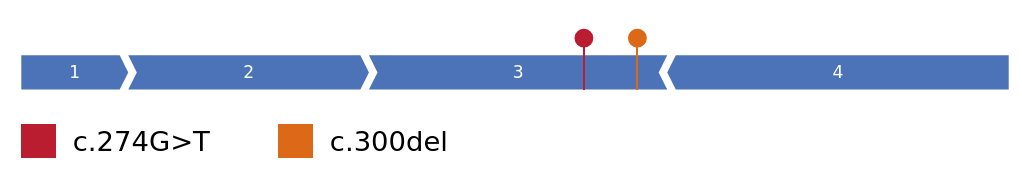
\includegraphics[scale=0.82]{images/SDHD.png}\\}
  \captionof{figure}{Transcript NM\_003002.4 for SDHD, with two variants}
  }

  % SHD noncoding
  \headerbox{SDHD (NM\_003002.4),  non coding}{name=SDHDnon,column=1,span=2,below=SDHD} {
  \captionsetup{labelformat=empty,margin=0.6cm}
  \noindent{\centering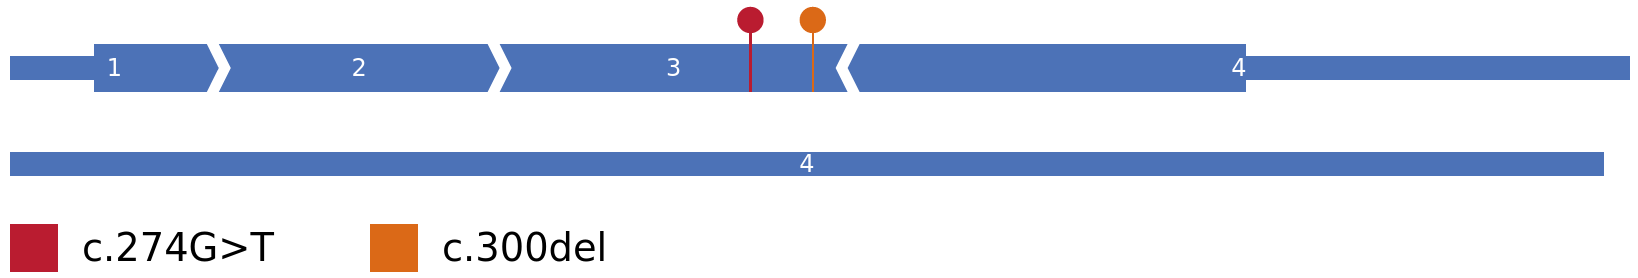
\includegraphics[width=0.95\linewidth]{images/SDHD-non.png}\\}
  \captionof{figure}{Transcript NM\_003002.4 for SDHD, with two variants}
  }

  % DMD figure
  \headerbox{DMD, schematic}{name=DMD,column=1,span=2,below=SDHDnon} {
  \captionsetup{labelformat=empty,margin=0.6cm}
  \noindent{\centering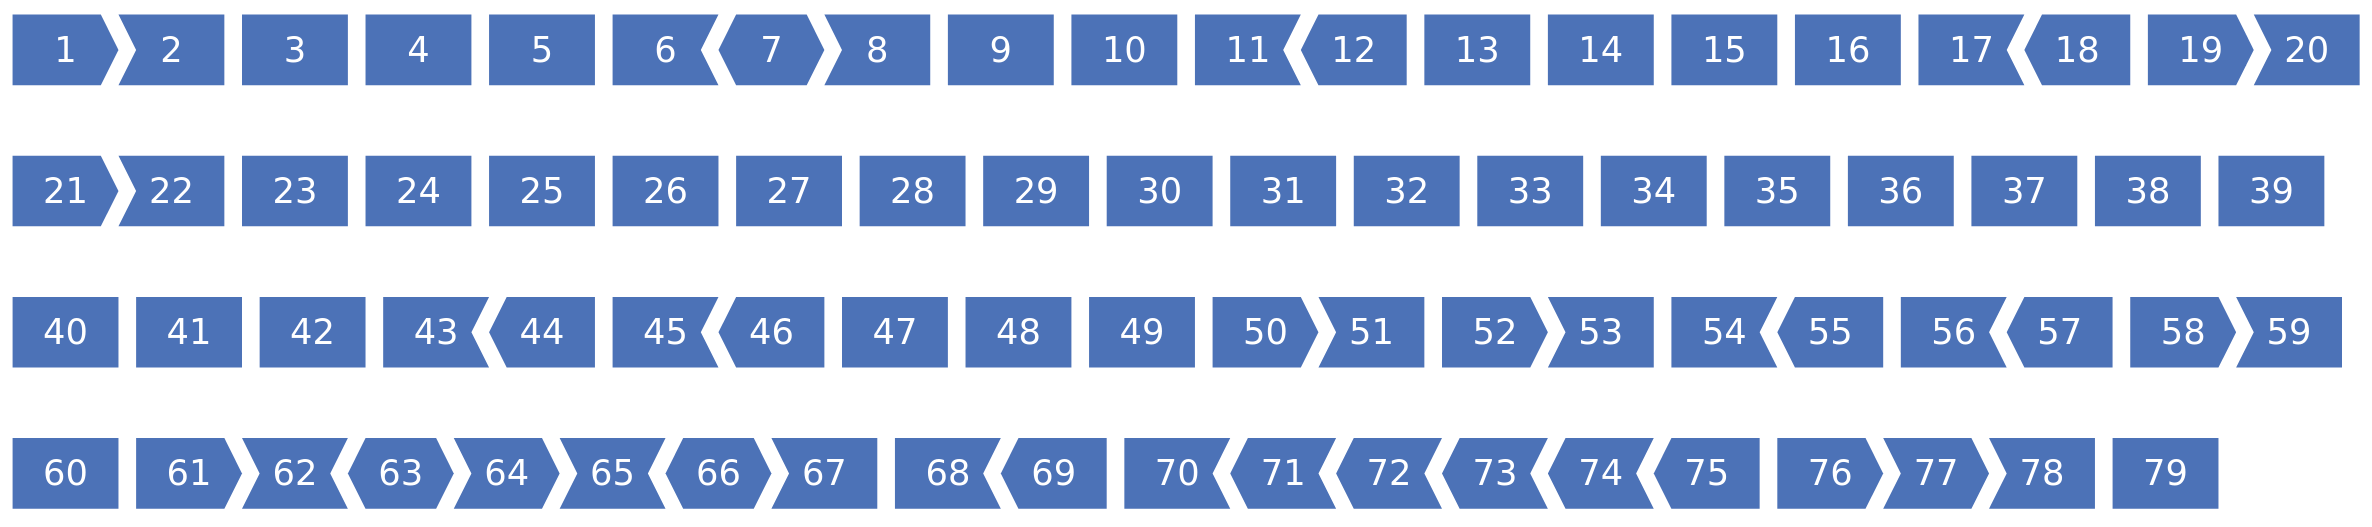
\includegraphics[width=0.95\linewidth]{images/DMD-schematic.png}\\}
  \captionof{figure}{Schematic representation of the coding region of \textit{Dystrophin}}
  }

  % CYLD figure
  \headerbox{CYLD, with variants from ClinVar}{name=CYLD,column=0,span=3,below=MM} {
  \captionsetup{labelformat=empty,margin=0.6cm}
  \noindent{\centering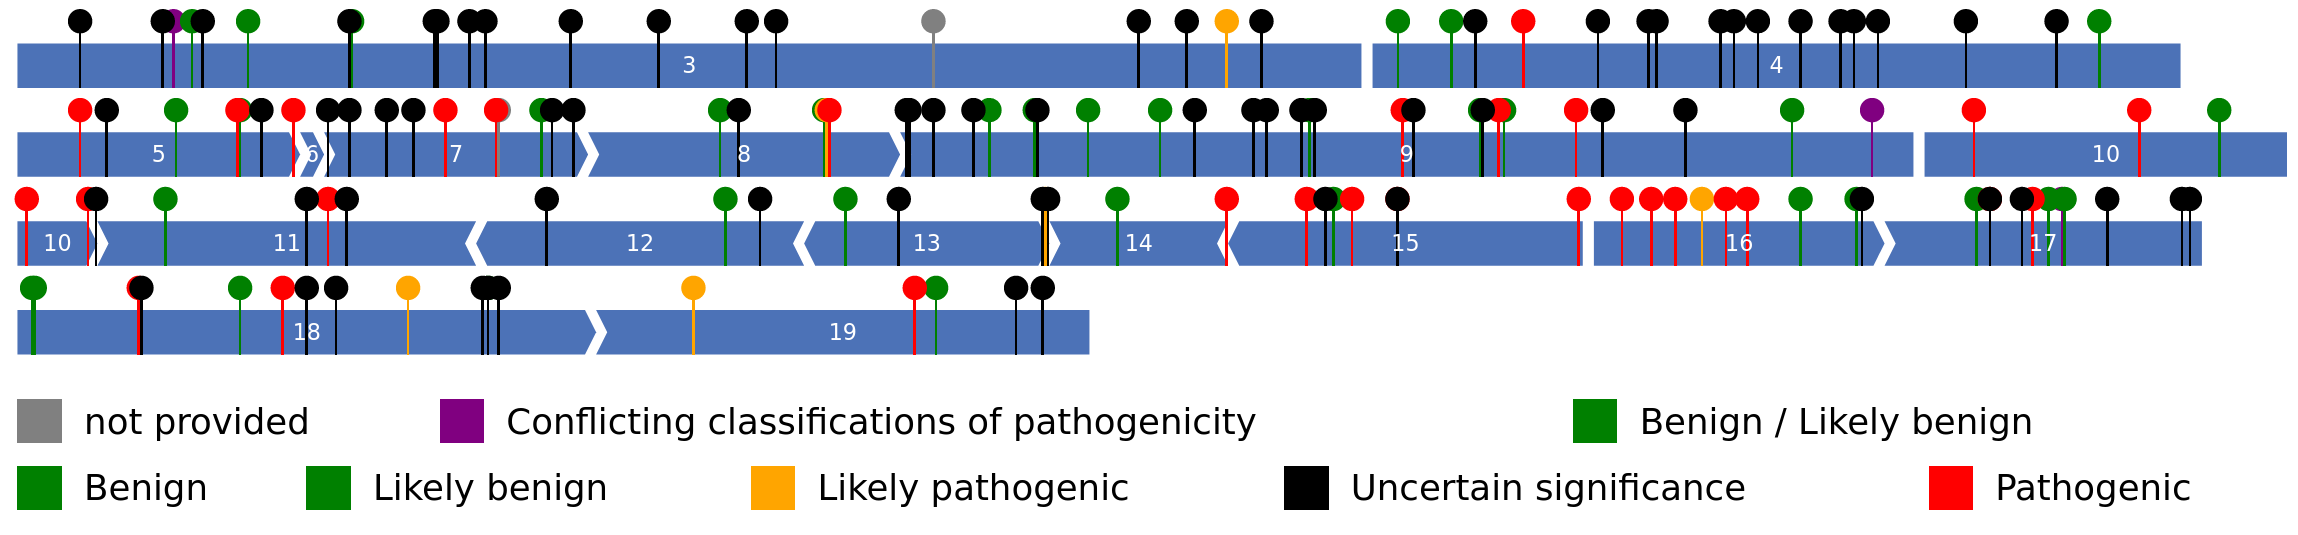
\includegraphics[width=0.95\linewidth]{images/CYLD.png}\\}
  \captionof{figure}{Transcript NM\_001378743.1 of CYLD, with all ClinVar variants by category}
  }

%%%%%%%%%%%%%%%%%%%%%%%%%%%%%%%%%%%%%%%%%%%%%%%%%%%%%%%%%%%%%%%%%%%%%%%%%%%%%%
  \headerbox{References}{name=ref,column=2,above=bottom} {
%%%%%%%%%%%%%%%%%%%%%%%%%%%%%%%%%%%%%%%%%%%%%%%%%%%%%%%%%%%%%%%%%%%%%%%%%%%%%%
    \tiny
    \begin{enumerate}[itemsep=-0.3ex,leftmargin=0.29cm]
      \item Lefter, M., et al. "Mutalyzer 2: next generation HGVS nomenclature checker, Bioinformatics (2021). https://doi.org/10.1093/bioinformatics/btab051
    \end{enumerate}
  }

%%%%%%%%%%%%%%%%%%%%%%%%%%%%%%%%%%%%%%%%%%%%%%%%%%%%%%%%%%%%%%%%%%%%%%%%%%%%%%
\headerbox{Contact}{name=contact,column=1, aligned=ref}
%%%%%%%%%%%%%%%%%%%%%%%%%%%%%%%%%%%%%%%%%%%%%%%%%%%%%%%%%%%%%%%%%%%%%%%%%%%%%%
  {
  \begin{center}
  \textbf{RedmarvandenBerg@lumc.nl}\linebreak
  \textbf{DCRT@lumc.nl}\linebreak
%\linebreak\linebreak\linebreak\linebreak
  \end{center}
  }


%%%%%%%%%%%%%%%%%%%%%%%%%%%%%%%%%%%%%%%%%%%%%%%%%%%%%%%%%%%%%%%%%%%%%%%%%%%%%%
\headerbox{QR Code}{name=qr,column=0,aligned=ref}
%%%%%%%%%%%%%%%%%%%%%%%%%%%%%%%%%%%%%%%%%%%%%%%%%%%%%%%%%%%%%%%%%%%%%%%%%%%%%%
  {
  %hfill to align right: https://tex.stackexchange.com/questions/55472/how-to-make-text-aligned-left-center-right-in-the-same-line
  \vspace{-0.3em}
  \begin{center}
  %\includegraphics[width=0.25\linewidth]{images/meegid_poster2016.png}
  % 
\includegraphics[width=0.25\linewidth]{images/meegid_heidelberg_poultry.png}
  \end{center}
  }
\end{poster}

\end{document}

